\documentclass[11pt,letterpaper]{article}
\usepackage[lmargin=1in,rmargin=1in,tmargin=1in,bmargin=1in]{geometry}
\usepackage{../style/homework}
\setbool{quotetype}{true} % True: Side; False: Under
\setbool{hideans}{false} % Student: True; Instructor: False

\usepackage{cancel} % Use Cancellations
\newcommand{\lh}{\stackrel{\text{L.H.}}{=}} % L'Hopital Equal

% -------------------
\begin{document}

\homework{1: Due 02/01}{And I knew exactly what to do\dots but in a much more real sense, I had no idea what to do.}{Michael Scott, The Office}

% Problem 1
\problem{10} Showing all your work and fully justifying your reasoning, compute the following:
	\begin{2enumerate}
	\item $\ds \lim_{x \to -6} \dfrac{x^2 + 3x - 18}{x^2 + 5x - 6}$
	\item $\ds \lim_{n \to \infty} \dfrac{2n^2 - 35n + 17}{6n^2 + 19n - 49}$
	\item $\dfrac{d}{dx} \, \ln \left(x \cos x \right)$
	\item $\ds \int_0^1 \dfrac{x}{x + 1} \;dx$
	\end{2enumerate} \pspace

\sol 
\begin{enumerate}[(a)]
\item 
	\[
	\lim_{x \to -6} \dfrac{x^2 + 3x - 18}{x^2 + 5x - 6}= \lim_{x \to -6} \dfrac{(x - 3)(x + 6)}{(x - 1)(x + 6)}= \lim_{x \to -6} \dfrac{(x - 3) \cancel{(x + 6)}}{(x - 1) \cancel{(x + 6)}}= \lim_{x \to -6} \dfrac{x - 3}{x - 1}= \dfrac{-6 - 3}{-6 - 1}= \dfrac{-9}{-7}= \dfrac{9}{7}
	\] 
		\begin{center} OR \end{center}
	\[
	\lim_{x \to -6} \dfrac{x^2 + 3x - 18}{x^2 + 5x - 6} \lh \lim_{x \to -6} \dfrac{2x + 3}{2x + 5}= \dfrac{-12 + 3}{-12 + 5}= \dfrac{-9}{-7}= \dfrac{9}{7}
	\] \pspace

\item 
	\[
	\lim_{n \to \infty} \dfrac{2n^2 - 35n + 17}{6n^2 + 19n - 49}= \lim_{n \to \infty} \dfrac{2n^2 - 35n + 17}{6n^2 + 19n - 49} \cdot \dfrac{1/n^2}{1/n^2}= \lim_{n \to \infty} \dfrac{2 - \frac{35}{n} + \frac{17}{n^2}}{6 + \frac{19}{n} - \frac{49}{n^2}}= \dfrac{2 - 0 + 0}{6 + 0 - 0}= \dfrac{2}{6}= \dfrac{1}{3}
	\]
		\begin{center} OR \end{center}
	\[
	\lim_{n \to \infty} \dfrac{2n^2 - 35n + 17}{6n^2 + 19n - 49} \lh \lim_{n \to \infty} \dfrac{4n - 35}{12n + 19} \lh \lim_{n \to \infty} \dfrac{4}{12}= \dfrac{1}{3}
	\] \pspace

\item 
	\[
	\dfrac{d}{dx} \, \ln \left(x \cos x \right)= \dfrac{1}{x \cos x} \cdot (\cos x - x \sin x)= \dfrac{\cos x - x \sin x}{x \cos x}= \dfrac{\cos x}{x \cos x} - \dfrac{x \sin x}{x \cos x}= \dfrac{1}{x} - \tan x
	\] \pspace

\item 
	\[
	\int_0^1 \dfrac{x}{x + 1} \;dx= \int_0^1 \dfrac{(x + 1) - 1}{x + 1} \;dx= \int_0^1 \left( 1 - \dfrac{1}{x + 1} \right) \;dx= x - \ln|x + 1| \bigg|_0^1= (1 - \ln 2) - (0 - \ln 1)= 1 - \ln 2
	\]
		\begin{center} OR \end{center}
	\[
	\int_0^1 \dfrac{x}{x + 1} \;dx \quad {u= x + 1 \atop du= dx} \quad \int_1^2 \dfrac{u - 1}{u} \;du= \int_1^2 \left(1 - \frac{1}{u} \right) \;du= u - \ln|u| \bigg|_1^2= (2 - \ln 2) - (1 - \ln 1)= 1 - \ln 2
	\]
\end{enumerate}



\newpage



% Problem 2
\problem{10} Recall that a sequence $\{ a_n \}$ is increasing if $a_{n+1} \geq a_n$ for all $n$ and the sequence is decreasing if $a_{n+1} \leq a_n$ for all $n$. A sequence $\{ a_n \}$ is called bounded above (below) if there exists $M \in \mathbb{R}$ such that $a_n \leq M$ ($a_n \geq M$) for all $n$. The \textit{Monotone Convergence Theorem} states the following: if $\{ a_n \}$ is either increasing or decreasing, i.e. is `monotone', and bounded above or below, respectively, then $\{ a_n \}$ converges. Now consider the sequence with $a_0= 2$ and given recursively via\dots
	\[
	a_{n+1}= \dfrac{1}{2} \left( a_n + \dfrac{5}{a_n} \right)
	\]

\begin{enumerate}[(a)]
\item Compute $a_1, a_2, a_3$. 
\item Compare your values in (a) to $\sqrt{5}$. What might you conjecture?
\item Explain why the Monotone Convergence Theorem implies that $\{ a_n \}$ has a limit. 
\item By (c), we know $L:= \ds \lim_{n \to \infty} a_n$ exists. Taking the limit in both sides of the recursive definition for $\{ a_n \}$, show that $L= \sqrt{5}$. 
\end{enumerate} 

\sol 
\begin{enumerate}[(a)]
\item We use the recurrence relation with $a_0= 2$. 
	\[
	\begin{aligned}
	a_1&= \dfrac{1}{2} \left( a_0 + \dfrac{5}{a_0} \right)= \dfrac{1}{2} \left( 2 + \dfrac{5}{2} \right)= \dfrac{1}{2} \cdot 4.5= 2.25 \\
	a_2&= \dfrac{1}{2} \left( a_1 + \dfrac{5}{a_1} \right)= \dfrac{1}{2} \left(2.25 + \dfrac{5}{2.25} \right)= \dfrac{1}{2} \cdot 4.47222= 2.23611 \\
	a_3&= \dfrac{1}{2} \left( a_2 + \dfrac{5}{a_2} \right)= \dfrac{1}{2} \left( 2.23611 + \dfrac{5}{2.23611} \right)= \dfrac{1}{2} \cdot 4.47214= 2.23607
	\end{aligned}
	\] 

\item We have $\sqrt{5} \approx 2.23607$. Based on the data from (a), we might conjecture (perhaps very foolishly based on so little evidence) that $a_n \to \sqrt{5}$ as $n \to \infty$. 

\item Based on the data above, it seems that the sequence $\{ a_n \}$ is decreasing for $n \geq 2$ because $a_3 < a_2$. Furthermore, it seems that the sequence $\{ a_n \}$ is bounded (below)---$a_n \geq 0$. If both these are true, then the sequence $\{ a_n \}$ is monotone decreasing. But then by the Monotone Convergence Theorem, $\{ a_n \}$ would converge to a limit, say $L$. [We prove this thoroughly at the end of the homework.]

\item By (c), we that $L:= \ds \lim_{n \to \infty} a_n$ exists. But then we also have $L:= \ds \lim_{n \to \infty} a_{n + 1}$. Moreover, because $a_n > 0$ for all $n$, we know that $L > 0$. Now\dots
	\[
	\begin{gathered}
	a_{n+1}= \dfrac{1}{2} \left( a_n + \dfrac{5}{a_n} \right) \\
	\lim_{n \to \infty} a_{n+1}= \lim_{n \to \infty} \dfrac{1}{2} \left( a_n + \dfrac{5}{a_n} \right) \\
	L= \dfrac{1}{2} \left(L + \dfrac{5}{L} \right) \\
	2L^2= L^2 + 5 \\
	L^2= 5 \\
	L= \pm \sqrt{5} \\
	L= \sqrt{5}
	\end{gathered}
	\]
\end{enumerate}



\newpage



% Problem 3
\problem{10} The Intermediate Value Theorem states the following: if $f(x)$ is continuous on $[a, b]$ and $f(a) < c < f(b)$, then there exists an $x_0 \in (a, b)$ such that $f(x_0)= c$. Consider the function $f(x)= x^2 - 3x + 4$ on the interval $[-1, 5]$. 
	\begin{enumerate}[(a)]
	\item Give a sketch of $f(x)$ on the interval $[-1, 6]$. 
	\item Explain why $f(x)$ is continuous. 
	\item Explain why there is a $x_0 \in [-1, 6]$ such that $f(x_0)= 14$. 
	\item Find the $x_0 \in [-1, 6]$ such that $f(x_0)= 14$. 
	\end{enumerate} \pspace

\sol 
\begin{enumerate}[(a)]
\item 
	\[
	\fbox{
	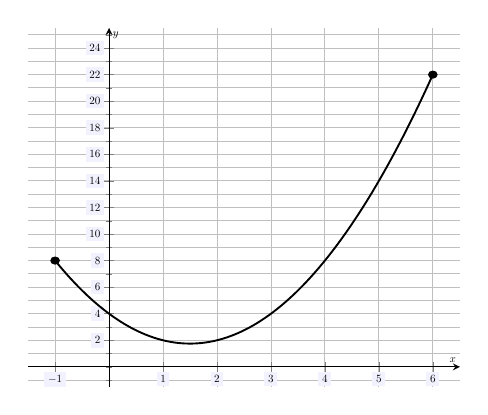
\begin{tikzpicture}[scale=0.8,every node/.style={scale=0.5}]
	\begin{axis}[
	grid=both,
	axis lines=middle,
	ticklabel style={fill=blue!5!white},
	xmin= -1.5, xmax=6.5,
	ymin= -1.5, ymax=25.5,
	xtick={-1,0,...,6},
	ytick={0,2,...,26},
	minor tick = {-26,...,26},
	xlabel=\(x\),ylabel=\(y\),
	]
	\addplot[line width=0.03cm,domain=-1:6,samples=100] ({x},{x^2 - 3*x + 4});
	\draw[fill=black] (-1,8) ellipse (0.08 and 0.27);
	\draw[fill=black] (6,22) ellipse (0.08 and 0.27);
	\end{axis}
	\end{tikzpicture}
	}
	\] \pspace

\item The function $f(x)$ is a polynomial. Hence, $f(x)$ is continuous on $\mathbb{R}$. In particular, it is continuous on $[-1, 6]$. \pspace

\item We have $f(-1)= 8$ and $f(6)= 22$. Clearly, $f(-1)= 8 < 14 < 22= f(6)$. By the Intermediate Value Theorem, there exists $x_0 \in [-1, 6]$ such that $f(x_0)= 14$. Alternatively, we can see that a horizontal line at $y= 14$ intersects the graph of $f(x)$. Note that from the graph above, there are also $x_0 \in [-1, 6]$ such that $f(x_0)= a$, where $a \in [\frac{7}{4}, 8)$---but the existence of such a $x_0$ does not follow from the Intermediate Value Theorem applied to $[-1, 6]$. \pspace

\item By (c), we know there exists $x_0 \in [-1, 6]$ such that $f(x_0)= 14$. But then\dots
	\[
	\begin{gathered}
	f(x_0)= 14 \\
	x_0^2 - 3x_0 + 4= 14 \\
	x_0^2 - 3x_0 - 10= 0 \\
	(x_0 - 5)(x_0 + 2)= 0
	\end{gathered}
	\]
But then $x_0= -2$ or $x_0= 5$. Clearly, $-2 \notin [-1, 6]$. Therefore, we have $x_0= 5$. We can confirm this: $f(5)= 5^2 - 3(5) + 4= 25 - 15 + 4= 14$. 
\end{enumerate}



\newpage



% Problem 4
\problem{10} The Mean Value Theorem states the following: if $f(x)$ is continuous on $[a, b]$ and differentiable on $(a, b)$, then there exists $c \in (a, b)$ such that $f(b) - f(a)= f'(c) \big( b - a \big)$. Consider the function $f(x)= x^3 + x^2 - 4x - 5$. Find the values $c \in [-1, 4]$ that satisfy the Mean Value Theorem. \pspace

\sol We first confirm that the Mean Value Theorem applies to $f(x)$. The function $f(x)$ is a polynomial. Therefore, $f(x)$ is continuous on $\mathbb{R}$ and infinitely differentiable on $\mathbb{R}$. In particular, $f(x)$ is continuous on $[-1, 4]$ and differentiable on $(-1, 4)$. By the Mean Value Theorem, there exists $c \in [-1, 4]$ such that $f(4) - f(-1)= f'(c) \big(4 - (-1) \big)$. We have\dots
	\[
	\begin{aligned}
	f(4)&= 4^3 + 4^2 - 4(4) - 5= 64 + 16 - 16 - 5= 59 \\[0.3cm]
	f(-1)&= (-1)^3 + (-1)^2 - 4(-1) - 5= -1 + 1 + 4 - 5= -1 \\[0.3cm]
	f'(x)&= 3x^2 + 2x - 4 \Rightarrow f'(c)= 3c^2 + 2c - 4
	\end{aligned}
	\]
But then we have\dots
	\[
	\begin{gathered}
	f(4) - f(-1)= f'(c) \big(4 - (-1) \big) \\[0.3cm]
	59 - (-1)= (3c^2 + 2c - 4) \cdot 5 \\[0.3cm]
	60= 5(3c^2 + 2c - 4) \\[0.3cm]
	12= 3c^2 + 2c - 4 \\[0.3cm]
	0= 3c^2 + 2c - 16 \\[0.3cm]
	0= (c - 2)(3c + 8)
	\end{gathered}
	\]
Therefore, $c= 2$ or $c= -\frac{8}{3}$. As $-\frac{8}{3} \notin (-1, 4)$, it must be that $c= 2$. Indeed, we have $f'(2)= 3(4) + 4 - 4= 12$, which has the same slope as the line connecting $\big(-1, f(-1) \big)$ and $\big(4, f(4) \big)$. 
	\[
	\fbox{
	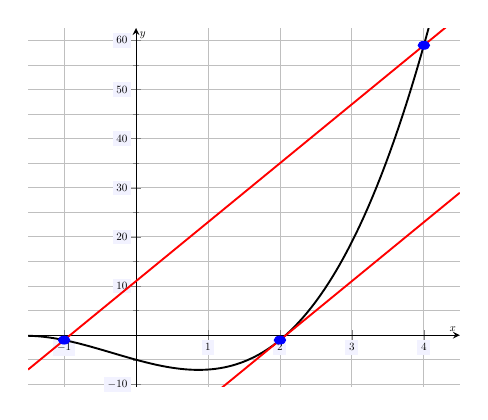
\begin{tikzpicture}[scale=0.8,every node/.style={scale=0.5}]
	\begin{axis}[
	grid=both,
	axis lines=middle,
	ticklabel style={fill=blue!5!white},
	xmin= -1.5, xmax=4.5,
	ymin= -10.5, ymax=62.5,
	xtick={-1,0,...,5},
	ytick={-10,0,...,60},
	minor tick = {-60,-55,...,60},
	xlabel=\(x\),ylabel=\(y\),
	]
	\addplot[line width=0.03cm,domain=-1.5:4.5,samples=100] ({x},{x^3 + x^2 - 4*x - 5});
	\addplot[line width=0.03cm,domain=-1.5:4.5,samples=100,red] ({x},{12*x + 11});
	\addplot[line width=0.03cm,domain=-1.5:4.5,samples=100,red] ({x},{12*x - 25});
	\draw[fill=black,blue] (-1,-1) ellipse (0.08 and 0.8133);
	\draw[fill=black,blue] (4,59) ellipse (0.08 and 0.8133);
	\draw[fill=black,blue] (2,-1) ellipse (0.08 and 0.8133);
	\end{axis}
	\end{tikzpicture}
	}
	\]



\newpage



{\bfseries Problem 2 (Continued).} We prove that the Monotone Convergence Theorem can be used to show that $\{ a_n \}$ converges to $\sqrt{5}$. We shall show that $a_n$ (or a tail of the sequence) is decreasing and bounded below. \pspace

{\itshape Bounded Below.} We need to show that there is an $M \in \mathbb{R}$ such that $M \leq a_n$ for all $n$. We shall show that $a_n \geq \sqrt{5}$ for all $n \geq 1$. We first show that $a_n$ is positive, i.e. $a_n \geq 0$, for all $n$ by induction. Clearly, $a_0= 2 > 0$. Assume that $a_n$ is positive. We need show that $a_{n+1}$ is positive. But\dots
	\[
	a_{n+1}= \dfrac{1}{2} \left( a_n + \dfrac{5}{a_n} \right)
	\]
But then $a_{n+1}$ is formed from the quotient, sum, and product of positive real numbers. Therefore, $a_{n+1}$ is positive. By induction, $a_n > 0$ for all $n$, i.e. $a_n$ is positive for all $n$. In fact, this shows that $\{ a_n \}$ is bounded below (by $M= 0$). \pspace

Because $a_n > 0$ for all $n$, $a_n \geq \sqrt{5}$ if and only if $a_n^2 \geq 5$. Now for $n \geq 1$, we have\dots
	\[
	a_{n+1}^2= \left( \dfrac{1}{2} \left(a_n + \dfrac{5}{a_n} \right) \right)^2= \left( \dfrac{a_n + \frac{5}{a_n}}{2} \right)^2 \geq a_n \cdot \dfrac{5}{a_n}= 5
	\]
We have used the fact that for all $x, y \in \mathbb{R}$, $\left( \frac{x + y}{2} \right)^2 \geq xy$. To see this, observe\dots
	\[
	\left( \dfrac{x + y}{2} \right)^2 - xy= \dfrac{x^2 + 2xy + y^2}{4} - xy= \dfrac{x^2 + 2xy + y^2}{4} - \dfrac{4xy}{4}= \dfrac{x^2 - 2xy + y^2}{4}= \dfrac{(x - y)^2}{4}= \left( \dfrac{x - y}{2} \right)^2 \geq 0
	\]
But then $\left( \frac{x + y}{2} \right)^2 \geq xy$. The above result then follows by taking $a= a_n$ and $b= \frac{5}{a_n}$. Because $a_{n+1}^2 \geq 5$ for all $n$, we know $a_{n+1} \geq 5$ for all $n$. \pspace

{\itshape Decreasing.} We show that $\{ a_n \}$ is decreasing for $n \geq 1$. To prove this, we show that $a_{n+1} - a_n \leq 0$, i.e. $a_n - a_{n+1} \geq 0$. For $n \geq 1$, we know that $a_n^2 \geq 5$ so that\dots
	\[
	\begin{aligned}
	a_n - a_{n+1}&= a_n - \dfrac{1}{2} \left( a_n + \dfrac{5}{a_n} \right) \\
	&= a_n - \dfrac{a_n}{2} - \dfrac{5}{2a_n} \\
	&= \dfrac{a_n}{2} - \dfrac{5}{2a_n} \\
	&= \dfrac{a_n^2}{2a_n} - \dfrac{5}{2a_n} \\
	&= \dfrac{a_n^2 - 5}{2a_n} \geq \dfrac{0}{2a_n} = 0
	\end{aligned}
	\]
But then $a_n - a_{n+1} \geq 0$ so that $\{ a_n \}$ is decreasing for $n \geq 1$. \pspace

Therefore, the sequence $\{ a_n \}_{n \geq 1}$ is decreasing and bounded below. Therefore, by the Monotone Convergence Theorem, the sequence $\{ a_n \}_{n \geq 1}$ converges. The sequence $\{ a_n \}_{n \geq 0}$ has a limit if and only if $\{ a_n \}_{n \geq 1}$ has a limit; if so, they have the same limit. Therefore, $\{ a_n \}_{n \geq 0}$ has a limit, $L$. 


\end{document}